% !TeX root = ../main.tex

\chapter{基于深度学习的时间序列异常检测框架设计与实现}
\label{cha:intro}
本章主要介绍本文实现的基于深度学习的时间序列异常检测框架,对执行流程和各个部分的设计进行详细说明。
\section{框架设计}
本文实现的基于深度学习的时间序列异常检测框架如图~\ref{fig:part1_overview}所示

\begin{figure}[H]
    \centering
    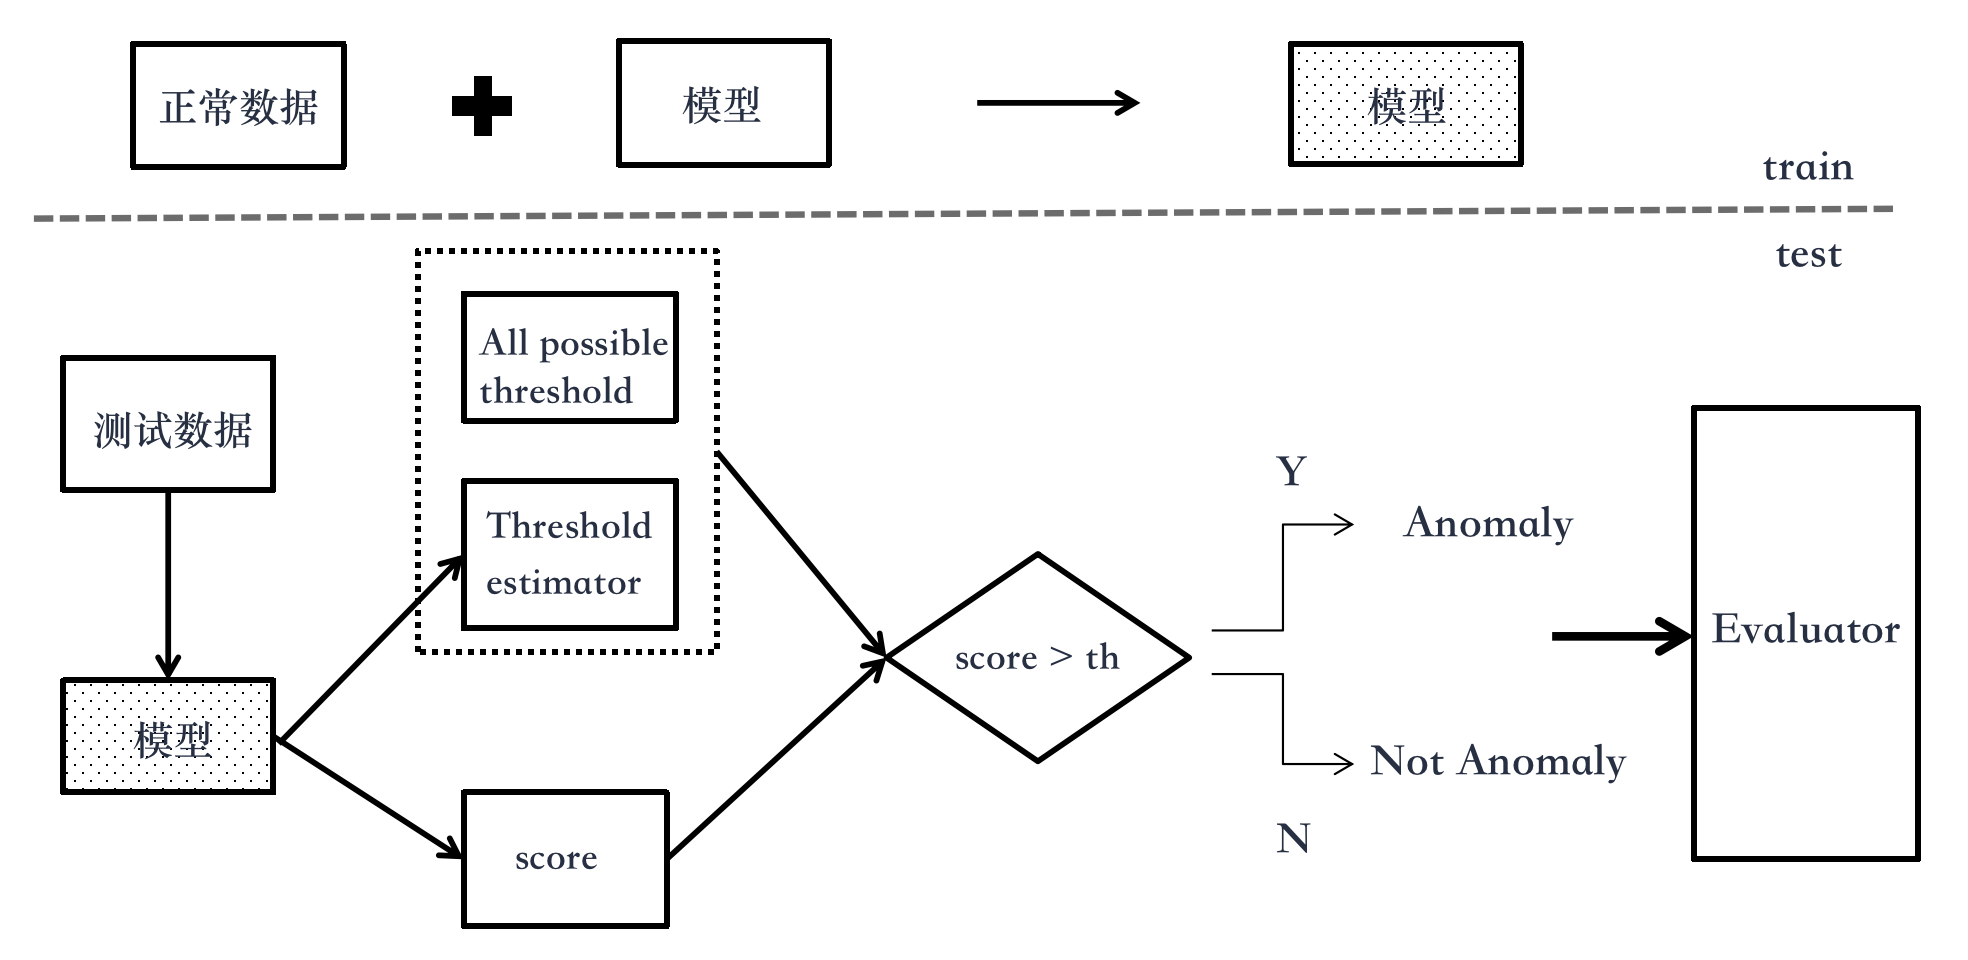
\includegraphics[width=\textwidth]{part1_overview.png}
    \caption{基于深度学习的时间序列异常检测框架}
    \label{fig:part1_overview}
  \end{figure}

我们的框架分为训练和测试两种运行模式。

在训练模式中,我们需要先用正常数据结合某个特定的模型训练出一个适用于该数据集的模型。然后在测试模式中时,模型对于每条数据会输出一个异常分数表示它的异常程度,通常情况下我们还需要模型来提供一个阈值,当异常程度>给定阈值时,认为该条数据是异常,否则认为正常,然后送到评估模块进行评估结果,或者我们枚举所有可能的阈值对结果进行评估,这样可以衡量模型的上限。

接下来分别对系统的几个关键部分进行阐述。

\section{数据集选择}
我们选择了在SMD(Server Machine Dataset)\cite{su2019robust}数据集上完成实验。其是从国内某互联网公司收集

\section{算法选择模块}
\section{动态阈值选取模块}
\section{评价模块}
\section{运行结果}


